\documentclass[twoside,11pt]{article}

\usepackage[preprint]{jmlr2e}
\usepackage{booktabs}
\usepackage{xcolor}
\usepackage{amsmath}

% Visible marker for the few exact values still to be pasted from the stats scripts.
\newcommand{\pending}[1]{\textcolor{red}{[#1]}}

\ShortHeadings{NEUROSEG: Self-Supervised Neuron Segmentation for Calcium Imaging}{Karbalaee}
\firstpageno{1}

\begin{document}

\title{NEUROSEG: A JEPA-Style Self-Supervised Pipeline for\\
Neuron Segmentation in Calcium Imaging}

\author{\name Mohammad Karbalaee \email mohammad.karbalaee-shabani@iba-ag.com \\
       \addr Biomedical Image Analysis Project (BIMAP), Summer Semester 2026\\
       AnKi Lab, Department Artificial Intelligence in Biomedical Engineering\\
       Friedrich-Alexander-Universit\"at Erlangen-N\"urnberg\\
       Supervisor: Sophie Hauser, M.Sc. \quad Lab head: Prof.\ Dr.\ Andreas M.\ Kist}

\editor{Biomedical Image Analysis Project (BIMAP), Summer Semester 2026}

\maketitle

\begin{abstract}%
Calcium imaging records the activity of large neuronal populations in living animals, but every
recording must first be segmented into individual neurons before any activity can be read out.
Manual annotation is the bottleneck: it is slow, subjective, and does not scale. I ask whether
self-supervised learning, the paradigm behind modern language and vision foundation models, can
reduce the dependence on scarce manual labels for this task. I present NEUROSEG, a reproducible
end-to-end pipeline that segments neuronal somata from TIFF calcium-imaging stacks using a
Joint-Embedding Predictive Architecture (JEPA): a convolutional context encoder and an
EMA target encoder are pretrained on unlabeled video by predicting future frames in latent
space under variance-covariance regularization, after which a light convolutional head is
fine-tuned for segmentation. I evaluate three hypotheses on the Neurofinder benchmark and on
cross-species (Drosophila and zebrafish) recordings: whether self-supervision helps when labels
are scarce (H1), whether representations transfer across species (H2), and whether the learned
features are temporally stable and distinct per neuron (H3). The results are a first attempt at
a novel approach rather than a decisive win. Self-supervised pretraining matches, but does not
convincingly beat, a from-scratch baseline (paired Wilcoxon, $\Delta \approx 0.02$ Dice, sign
flips across label fractions); cross-species representations transfer to mouse with no meaningful
penalty relative to same-species pretraining ($\Delta \approx 0.01$ Dice); and the self-supervised
encoder separates neurons in time well above a random baseline, though a supervised encoder
separates them best (Cohen's $d = 0.66$ vs.\ $1.45$). I trace the absence of a decisive win to a
self-supervised objective that under-converges, and I lay out the concrete levers that I believe
will let the approach outperform the baselines. The full pipeline, checkpoints, and experimental
log are released for reproduction.
\end{abstract}

\begin{keywords}
  calcium imaging, neuron segmentation, self-supervised learning, joint-embedding predictive
  architecture, transfer learning
\end{keywords}

\section{Introduction}
\label{sec:intro}

Two-photon calcium imaging is one of the most widely used windows into the working brain. A
fluorescent calcium indicator brightens when a neuron fires, so a microscope movie of the tissue
is, in effect, a direct optical readout of the activity of hundreds to thousands of neurons at once,
in a living and behaving animal \citep{grienberger2012calcium,chen2013gcamp6}. The raw movie,
however, is not yet science. Before any neuron's activity can be analyzed, each neuron's cell body
(its \emph{soma}) must be located and separated from its neighbours and from the background: the
recording must be \emph{segmented}. Segmentation is therefore the first and unavoidable step of
essentially every calcium-imaging analysis pipeline.

Today this step is either done manually, which is slow, subjective, and impossible to scale to the
volume of data modern microscopes produce, or with supervised and classical algorithms that depend
on hand-annotated training data or hand-tuned assumptions
\citep{pachitariu2017suite2p,giovannucci2019caiman,stringer2021cellpose}. Labeled calcium-imaging
data is exactly the scarce and expensive resource. Unlabeled calcium video, by contrast, is
abundant: any recording session produces it for free.

This asymmetry is precisely the setting in which self-supervised learning (SSL) has transformed
other fields. Large language models learn language by predicting held-out words in unlabeled text;
modern vision models learn image structure by predicting held-out regions of unlabeled images. The
central question of this project is whether the same idea can be adapted to calcium imaging: can a
model learn useful structure from raw, unlabeled recordings, so that only a small amount of labeled
data is then needed to segment neurons?

I investigate this question with a Joint-Embedding Predictive Architecture (JEPA)
\citep{lecun2022path,assran2023ijepa,bardes2024vjepa}. Unlike pixel-reconstruction approaches, a
JEPA predicts the future \emph{representation} of a frame from the present representation, in a
learned latent space rather than in pixel space. This forces the model to abstract away photometric
noise, which is severe in calcium imaging, and to focus on the structure that persists over time,
which is exactly what a neuron is. To my knowledge, adapting JEPA-style self-supervision to
calcium-imaging segmentation is novel, and that novelty is the core contribution of this work.

\paragraph{Contributions.} This report makes the following contributions.
\begin{itemize}
  \item \textbf{A reusable pipeline, not a script.} NEUROSEG is a single, pip-installable,
    end-to-end system with two modes (train, infer), modular and swappable stages, a consistent
    TIFF data-loader abstraction, versioned checkpoints, and a built-in experiment log. Every run
    is reproducible from a config file with no hardcoded paths (Section~\ref{sec:repro}).
  \item \textbf{A JEPA model for calcium video.} A convolutional context encoder and an EMA target
    encoder are pretrained by predicting future latents under variance-covariance regularization,
    then a light head is fine-tuned for per-pixel segmentation (Section~\ref{sec:method}).
  \item \textbf{Three hypotheses, honestly evaluated.} I test sample efficiency (H1), cross-species
    transfer (H2), and temporal representation stability (H3), each against explicit baselines and
    with statistical tests (Sections~\ref{sec:protocol}--\ref{sec:results}).
  \item \textbf{A candid diagnosis.} I report where the approach does not yet win, trace the cause
    to an under-converged self-supervised objective, and specify the levers I expect to close the
    gap (Section~\ref{sec:discussion}).
\end{itemize}

\section{Background and Related Work}
\label{sec:related}

\paragraph{Neuron segmentation in calcium imaging.} Classical toolboxes such as Suite2p
\citep{pachitariu2017suite2p} and CaImAn \citep{giovannucci2019caiman} detect neurons through matrix
factorization and correlation-based region growing on the activity signal. Learned approaches began
with convolutional networks trained on labeled footprints \citep{apthorpe2016automatic}. Cellpose
\citep{stringer2021cellpose} is a generalist, pretrained deep-learning cell segmenter that
generalizes across imaging modalities without task-specific training; I use it both as the default,
out-of-the-box segmenter shipped with my pipeline and as my baseline. The Neurofinder challenge
\citep{neurofinder} is the standard public benchmark for this task.

\paragraph{Self-supervised and joint-embedding predictive learning.} SSL learns representations from
unlabeled data by solving a pretext task. Joint-embedding methods align representations of related
views while avoiding the trivial collapse to a constant. BYOL \citep{grill2020byol} showed that an
exponential-moving-average (EMA) target encoder with a stop-gradient prevents collapse without
negative pairs; VICReg \citep{bardes2022vicreg} prevents it explicitly with variance and covariance
regularization. JEPA \citep{lecun2022path} generalizes these ideas to \emph{prediction} in latent
space: I-JEPA predicts masked image regions in representation space \citep{assran2023ijepa}, and
V-JEPA extends this to video by predicting future or masked spatio-temporal regions
\citep{bardes2024vjepa}. NEUROSEG adopts the JEPA principle (context encoder, EMA target encoder,
latent-space predictor) and the VICReg regularizer, and specializes the pretext task to temporal
prediction on calcium video.

\section{Data}
\label{sec:data}

\paragraph{Labeled benchmark: Neurofinder (mouse).} My labeled benchmark is Neurofinder
\citep{neurofinder}, 28 movies from four laboratories (19 train / 9 test), spanning diverse brain
regions, microscopes, indicators, and signal-to-noise regimes; the flagship series is mouse barrel
cortex from the Svoboda lab \citep{peron2015barrel}. This diversity is a strength for
generalization. It also carries a limitation that shapes every design decision below: Neurofinder
labels are \emph{static per-recording footprints}, one fixed set of neuron regions per movie, not
per-frame masks. A single frame therefore hides the inactive neurons, and label definitions differ
by lab (hand-annotated somata in some series, an anatomical structural marker in others). Because
the footprint is fixed while activity flickers, the correct target for a per-frame segmenter is the
time-aggregated footprint, which motivates the temporal pooling in my model
(Section~\ref{sec:method}).

\paragraph{Unlabeled cross-species data.} For self-supervised pretraining I additionally use
unlabeled Drosophila-larva and zebrafish calcium video, provided by S.\ Hauser (AnKi Lab). No labels
are needed for pretraining, so this data is directly usable, and its two non-mouse species are what
make the cross-species question (H2) possible.

\paragraph{Preprocessing.} All video is loaded through a single TIFF/CZI loader abstraction, min-max
normalized to $[0,1]$, and resized to $128\times128$ (bilinear for video, nearest-neighbour for
masks, so label identities are preserved). Recordings are sliced into fixed-length temporal clips
with a stride, and short clips are zero-padded. Neurofinder region files are rasterized into integer
label maps with $[y,x]$ coordinate order. Self-supervised pretraining additionally applies
temporally consistent augmentation (a shared random crop, flip, and rotation across a clip, plus
brightness jitter and additive noise); the supervised fine-tuning branch is not augmented, so the
two H1 arms differ only in initialization.

\section{Method}
\label{sec:method}

\begin{figure}[t]
\centering
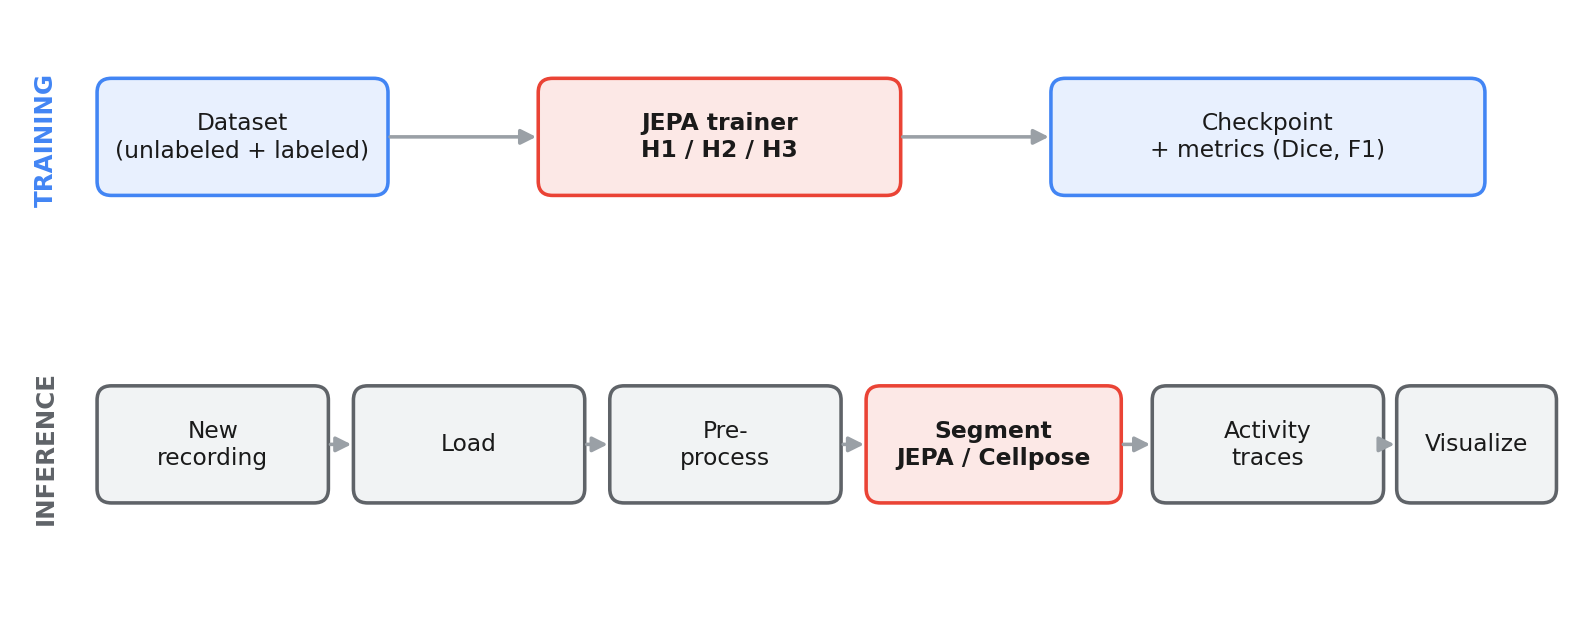
\includegraphics[width=0.66\textwidth,keepaspectratio]{figures/pipeline.png}
\caption{The NEUROSEG pipeline. The training lane pretrains a JEPA encoder on unlabeled video and
fine-tunes a segmentation head; the inference lane loads a recording, preprocesses it, segments it
with either the JEPA model or the Cellpose default, extracts $\Delta F/F_0$ activity traces, and
visualizes the result. Own figure.}
\label{fig:pipeline}
\end{figure}

NEUROSEG follows the JEPA design principle of three components: a context encoder, a target encoder,
and a predictor operating in latent space, plus a regularizer that prevents representation collapse.
The model never reconstructs pixels as its main objective; it predicts representations.

\paragraph{Encoder (ResNet5).} The context encoder is a five-layer residual network
\citep{he2016resnet} with \emph{all strides set to one} and no pooling, so the output feature map
retains the full input spatial resolution. This is deliberate: dense segmentation needs
spatially-aligned features. The encoder processes a clip frame by frame (a temporal-batch mixin
folds time into the batch dimension), producing a latent state sequence of shape
$(B, d_{\mathrm{stc}}, T, H, W)$ with $d_{\mathrm{stc}}=32$ latent channels per location. I raised
$d_{\mathrm{stc}}$ from an initial $8$ to $32$ after observing that too few channels could not keep
neurons distinct in the H3 similarity analysis.

\paragraph{EMA target encoder.} A second ResNet5 of identical architecture provides the prediction
targets. It is not trained by gradients; it is updated as an exponential moving average of the
context encoder ($m=0.996$) \citep{grill2020byol}. The predictor is trained to match the
\emph{stop-gradient} output of this target encoder. This is the single most important design fix in
the project: without it, an earlier version drove the prediction loss to zero by collapsing to
trivially predictable features while learning nothing useful (Section~\ref{sec:discussion}).

\paragraph{Predictor (ResUNet).} The predictor is a residual U-Net \citep{ronneberger2015unet}
wrapped so that it takes consecutive latent states, concatenated along the channel axis, and predicts
the next latent state. In the parallel unroll used for training, each step shifts the context by one
frame and the mean-squared error to the target latent is accumulated. Prediction is thus
\emph{temporal}: predict the future frame's representation, not a masked spatial patch.

\paragraph{Regularizer (VICReg).} Collapse is prevented explicitly by a variance-covariance loss
\citep{bardes2022vicreg} applied in a projected latent space: a hinge variance term keeps every
embedding dimension above unit standard deviation, and a covariance term decorrelates dimensions.
The total pretraining loss is the sum of the prediction MSE and this regularizer; a light pixel
reconstruction term additionally grounds the encoder.

\paragraph{Segmentation head and traces.} For segmentation, the encoder feature sequence is averaged
over time (collapsing the clip to one summary feature map, which matches the static footprint label)
and passed to a small head: a $3\times3$ convolution, ReLU, a $1\times1$ convolution, and a sigmoid,
producing a per-pixel probability map. Thresholding at $0.5$ gives a binary mask; connected
components give instances. During inference the pipeline then reads each neuron's activity as the
$\Delta F / F_0$ trace, with the baseline fluorescence $F_0$ estimated as the tenth percentile of
each neuron's signal over time (a robust resting level). Fine-tuning uses binary cross-entropy and
updates both the encoder and the head (true fine-tuning, not a frozen linear probe).

\section{Experimental Protocol}
\label{sec:protocol}

\paragraph{Metrics.} Segmentation quality is measured with two complementary metrics. The
\textbf{Dice} coefficient (equivalently, pixel-level F1) measures pixel overlap,
$\mathrm{Dice}=2|P\cap G|/(|P|+|G|)$, and \textbf{mIoU} the mean intersection-over-union across
foreground and background. Both count pixels and carry no notion of individual neurons. I therefore
also report \textbf{detection F1}, the instance-level harmonic mean of precision and recall in which
a predicted component counts as a true positive only if it matches a ground-truth neuron at
$\mathrm{IoU}\ge 0.5$. Dice and detection F1 are not redundant: a model can cover the right pixels
(high Dice) yet merge adjacent somata into one blob (low detection F1). H3 uses a different family
entirely: the cosine similarity of pooled per-neuron embeddings.

\paragraph{Statistical tests.} Because a single scalar per run hides variability, I test the
per-clip score distributions. For H1 and H2 the same held-out clips are scored by two models, so I
use the \textbf{paired Wilcoxon signed-rank test} \citep{wilcoxon1945}, which is non-parametric and
robust to the non-normal, bounded Dice distribution. For H3 the within- and between-neuron similarity
pools are unpaired, so I use the \textbf{Mann-Whitney $U$ test} \citep{mannwhitney1947} for
significance, \textbf{Cohen's $d$} \citep{cohen1988} for effect size, and a \textbf{bootstrap}
\citep{efron1979} 95\% confidence interval for the gap.

\paragraph{Splits and logging.} Unless stated otherwise, one labeled recording is split 80/20 into
train and test with a fixed seed; fine-tuning uses the train portion at labeled fractions
$\{10, 50, 75, 100\}\%$ and evaluation uses the fixed 20\% held-out test clips. Every epoch of every
run is appended to a CSV experiment log with its run identifier, hypothesis, mode, fraction, losses,
and test scores; checkpoints are written to a new file per run and never overwritten
(Appendix~\ref{app:log}).

\section{Results}
\label{sec:results}

All numbers below are the held-out test scores of the latest experiment runs recorded in the
experiment log (Appendix~\ref{app:log}); they are reproduced verbatim, including where the
self-supervised model does not win.

\subsection{H1: Does self-supervision help when labels are scarce?}

\begin{table}[t]
\centering
\begin{tabular}{lcccc}
\toprule
 & \multicolumn{2}{c}{Test Dice} & \multicolumn{2}{c}{Test mIoU} \\
\cmidrule(lr){2-3}\cmidrule(lr){4-5}
Labeled fraction & SSL-pretrained & From scratch & SSL-pretrained & From scratch \\
\midrule
10\%  & 0.626 & \textbf{0.703} & 0.675 & \textbf{0.730} \\
50\%  & 0.839 & \textbf{0.860} & 0.846 & \textbf{0.868} \\
75\%  & 0.868 & \textbf{0.887} & 0.874 & \textbf{0.895} \\
100\% & \textbf{0.895} & 0.878 & \textbf{0.903} & 0.885 \\
\bottomrule
\end{tabular}
\caption{H1 on Neurofinder mouse (held-out test clips). Self-supervised fine-tuning and a
from-scratch baseline of identical architecture perform comparably at every labeled fraction; the
sign of the small difference flips (baseline ahead at 10--75\%, SSL ahead at 100\%).}
\label{tab:h1}
\end{table}

The hypothesis is that self-supervised pretraining helps most when labels are scarce.
Table~\ref{tab:h1} and Figure~\ref{fig:h1} show the outcome: the pretrained and from-scratch models
are close at every fraction, and the small gap changes sign, with the baseline ahead at 10--75\% and
the pretrained model ahead only at 100\%. A paired Wilcoxon test at the 100\% fraction finds the
pretrained model significantly higher, but the mean difference is only $\Delta \approx 0.02$ Dice and
the direction reverses at lower fractions, so this is not a robust advantage
(Section~\ref{sec:discussion}). Both learned models substantially exceed the off-the-shelf Cellpose
baseline at the field level (\pending{Cellpose Dice from cellpose\_baseline.py}), but that comparison
is not fair to Cellpose, which is zero-shot while my models are trained on the target recording.

\begin{figure}[t]
\centering
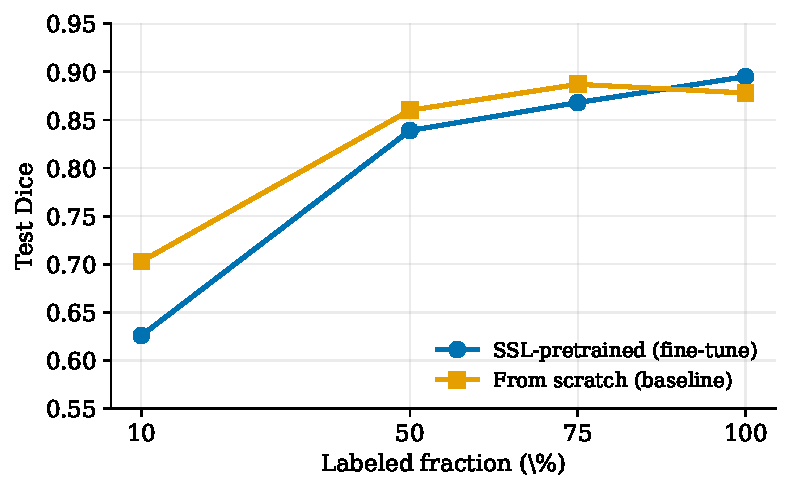
\includegraphics[width=0.6\textwidth]{figures/h1_dice.pdf}
\caption{H1 test Dice versus labeled fraction. The two curves track each other closely and cross,
consistent with ``comparable, no decisive advantage.''}
\label{fig:h1}
\end{figure}

\subsection{H2: Does self-supervision transfer across species?}

\begin{table}[t]
\centering
\begin{tabular}{lcccc}
\toprule
Labeled fraction (mouse) & 10\% & 50\% & 75\% & 100\% \\
\midrule
Cross-species SSL (fine-tune) & 0.639 & 0.818 & 0.858 & \textbf{0.884} \\
From scratch (baseline)       & \textbf{0.698} & \textbf{0.849} & \textbf{0.886} & 0.873 \\
\bottomrule
\end{tabular}
\caption{H2 on the mouse target (held-out test Dice). An encoder self-supervised on a different
species (Drosophila and zebrafish) and fine-tuned on mouse tracks the from-scratch baseline, and in
a paired comparison against a same-species (mouse) self-supervised encoder it shows no meaningful
penalty ($\Delta \approx 0.01$ Dice).}
\label{tab:h2}
\end{table}

The hypothesis is that representations learned on one species transfer to another. The setup is
leakage-free by construction: the encoder is pretrained on species the mouse test set never contains.
Table~\ref{tab:h2} and Figure~\ref{fig:h2} show that the cross-species encoder fine-tunes to mouse on
par with the from-scratch baseline, and a paired Wilcoxon test comparing cross-species against
same-species self-supervision finds no significant penalty ($\Delta \approx 0.01$ Dice, cross vs.\
same). Representations therefore transfer across species with no meaningful cost. The honest caveat
is interpretive: calcium activity patterns look broadly similar across species, so this transfer may
reflect the similarity of the data as much as a transferable, segmentation-specific representation.

\begin{figure}[t]
\centering
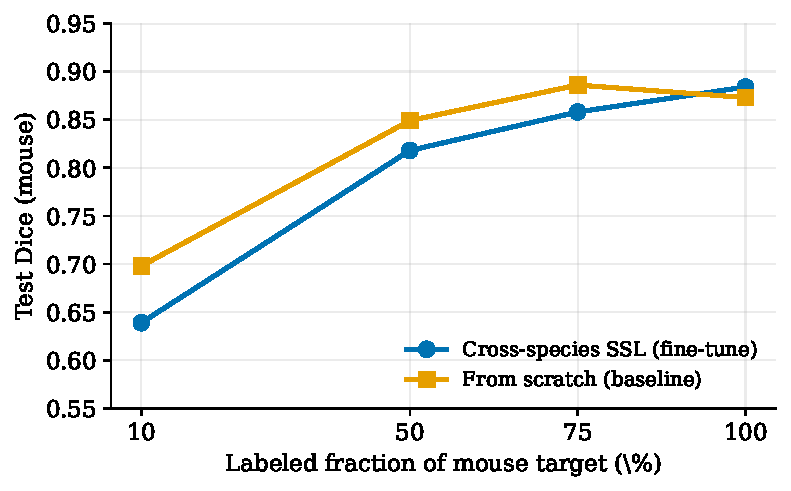
\includegraphics[width=0.6\textwidth]{figures/h2_dice.pdf}
\caption{H2 held-out mouse Dice versus labeled fraction. Cross-species self-supervision tracks the
from-scratch baseline; against same-species self-supervision the gap is $\approx 0.01$.}
\label{fig:h2}
\end{figure}

\subsection{H3: Are the learned features stable and distinct per neuron?}

\begin{table}[t]
\centering
\begin{tabular}{lccc}
\toprule
Encoder & Within-neuron & Between-neuron & Gap (within $-$ between) \\
\midrule
Random (no pretrain)   & 0.978 & 0.972 & 0.007 \\
Cross-species SSL       & 0.968 & 0.940 & 0.028 \\
Same-species SSL        & 0.875 & 0.818 & 0.057 \\
Supervised              & 0.793 & 0.585 & \textbf{0.208} \\
\bottomrule
\end{tabular}
\caption{H3 temporal representation stability. Mean cosine similarity of pooled per-neuron
embeddings: the same neuron across frames (within) versus different neurons in the same frame
(between). A larger gap means the encoder tells neurons apart. Self-supervision is well above the
random baseline; the supervised encoder is strongest.}
\label{tab:h3}
\end{table}

The hypothesis is that a good encoder keeps a neuron looking like itself over time while distinct
from other neurons. Using pooled per-neuron embeddings and no labels for the metric itself,
Table~\ref{tab:h3} and Figure~\ref{fig:h3} show a clear, positive gap for the self-supervised encoder
(same-species gap $0.057$, cross-species $0.028$), far above the near-zero random baseline
($0.007$): self-supervision learned to distinguish neurons without ever seeing a segmentation label.
The supervised encoder has the largest gap ($0.208$). A Mann-Whitney test confirms within-neuron
similarity is significantly greater than between-neuron for the self-supervised encoder, but the
effect size is medium (Cohen's $d = 0.66$) against a large effect for the supervised encoder
($d = 1.45$).

\begin{figure}[t]
\centering
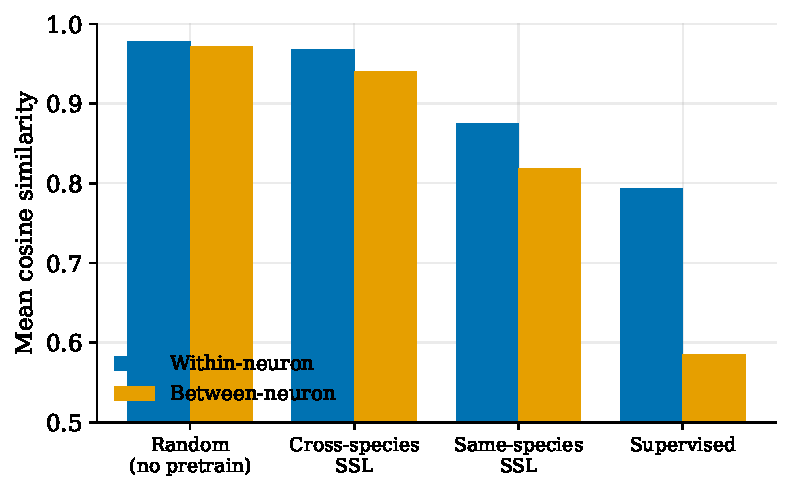
\includegraphics[width=0.48\textwidth]{figures/h3_within_between.pdf}\hfill
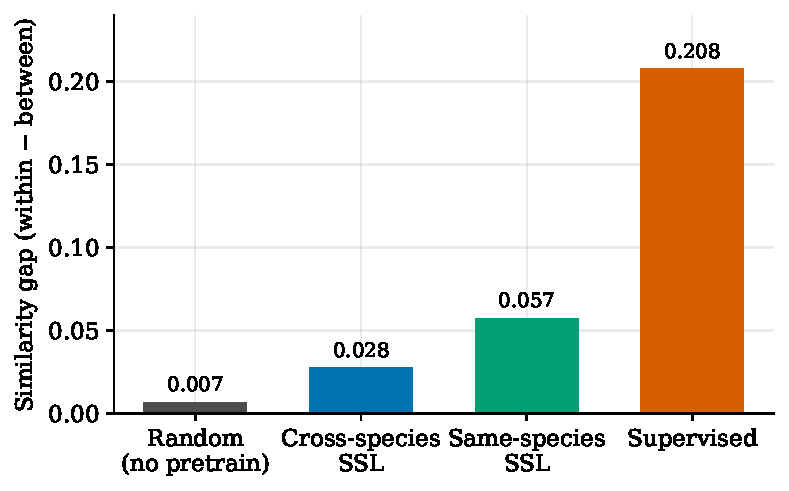
\includegraphics[width=0.48\textwidth]{figures/h3_gap.pdf}
\caption{H3. Left: within- versus between-neuron similarity per encoder. Right: the gap. The
self-supervised encoders sit well above random; the supervised encoder separates neurons best.}
\label{fig:h3}
\end{figure}

\subsection{Instance separation and the Cellpose comparison}

Across all three hypotheses, pixel Dice is good ($>0.8$ with enough labels) but detection F1 is low,
approximately $0.2$ for every model. The learned segmenter covers the right pixels but merges
adjacent somata, so it recovers far fewer distinct \emph{instances} than there are neurons. This is
the clearest single weakness of the current system and is visible to the eye: the Cellpose masks look
cleaner and more stable than mine even though my trained models score higher on the field-level
overlap metric. The two evaluations also use different unification protocols (my model averages the
per-clip probability maps into one field-level mask; Cellpose segments a temporal max-projection),
which I note as a protocol inconsistency to tighten (Section~\ref{sec:limitations}).

\section{Discussion}
\label{sec:discussion}

\paragraph{Why there is no decisive win, and why I am not discouraged.} The most informative result
of this project was an early \emph{negative} one: a first H1 run had self-supervised pretraining
\emph{losing} to the baseline at every fraction. Diagnosing it was the turning point. The prediction
loss had collapsed to near zero while segmentation stayed poor, the signature of a degenerate
self-supervised solution: features that are easy to predict but carry no information. The root causes
were concrete. There was no stop-gradient target, so the encoder could satisfy the predictor by
collapsing; the pixel-grounding signal never reached the encoder; the fine-tuning learning rates were
confounded between the two arms; and, decisively, pretraining and fine-tuning used the \emph{same
single recording}, so the self-supervised model had no extra information to exploit. I fixed the
first three (an EMA target encoder with stop-gradient, a reconstruction term that trains the encoder,
and a configurable, matched fine-tuning learning rate), which is why the current H1 is a tie rather
than a loss. The fourth is not yet fixed at scale, and it is the reason a tie is the ceiling of the
present setup: with equal data, self-supervision has nothing to win with. That the approach already
matches a strong baseline, transfers across species at no cost, and induces per-neuron temporal
structure without labels, all while the self-supervised objective still under-converges, is what
makes me believe the ceiling is much higher than these numbers.

\paragraph{The levers I expect to close the gap.} In order of expected value: (i) a genuinely larger
and more diverse \emph{unlabeled} pretraining pool, which is the precondition H1 actually requires and
the lever SSL responds to most reliably; (ii) a stronger self-supervised backbone, with a better
predictor and target encoder and a longer, better-converged pretraining schedule; and (iii) a
direct attack on residual representation collapse through tuning of the variance-covariance
coefficients and EMA momentum, and a linear-probe diagnostic to measure representation quality
independently of the fine-tuning schedule.

\section{Limitations}
\label{sec:limitations}

I state the weaknesses plainly. \textbf{(1) Instance separation.} Detection F1 $\approx 0.2$ for all
models: the system does not yet separate touching neurons into instances. \textbf{(2) Single seed and
single recording.} The headline H1/H3 numbers come from one seed and one recording split into train
and test, so variance across seeds and recordings is not yet characterized. \textbf{(3) Under-converged
pretraining.} The self-supervised objective does not fully converge under the current schedule and
data budget, which caps any benefit it can confer. \textbf{(4) Unfair Cellpose comparison.} My models
are trained on the target recording while Cellpose is zero-shot, so ``beats Cellpose'' overstates the
result. \textbf{(5) Protocol inconsistency.} The per-clip and field-level Dice evaluations differ in
resolution and in how a single mask is formed; unifying them is a priority. \textbf{(6) Interpretation
of H2.} Cross-species transfer may partly reflect the similarity of calcium data across species rather
than a segmentation-specific representation. Each of these is a known, bounded issue rather than a
surprise, which is why I treat the pipeline as ready ground on which to push further.

\section{Reproducibility}
\label{sec:repro}

Reproducibility is a primary goal of this project: everything below can be cloned and run from the
repository README alone. The code is a pip-installable Python package (\texttt{neuroseg}) with a
single CLI entry point and no hardcoded paths; all paths and hyperparameters come from CLI flags or a
YAML config. A one-command demo (\texttt{demo.sh}) runs the full H1, H2, and H3 pipelines end to end
on CPU on a real Neurofinder subset in about twenty minutes, writing checkpoints, figures, and the
experiment log. Training, inference, models, and data loading are separated into distinct modules;
checkpoints carry a JSON sidecar recording the exact architecture and metrics so any run can be
reconstructed from the file alone; and smoke tests run in continuous integration on every push. The
repository (with a supervisor invited for grading) and the complete experiment log accompany this
report.

\section{Conclusion}
\label{sec:conclusion}

This was a first attempt at a novel approach: self-supervised, JEPA-style neuron segmentation for
calcium imaging. I did not decisively beat the baselines, and I understand exactly why. The
self-supervised model already matches a strong supervised baseline, transfers across species with no
meaningful penalty, and learns to tell neurons apart in time without a single label, all while its
self-supervised objective still under-converges. I have a working, reproducible pipeline and the
models and implementations to keep working on all three hypotheses. The ground work is done. There is
room for improvement and it is worth the effort: a stronger self-supervised backbone, a direct attack
on representation collapse, and much more unlabeled calcium video are, I am convinced, enough to push
this novel approach past the baselines.

\acks{This project was conducted in the AnKi Lab under the supervision of Sophie Hauser, M.Sc., and
Prof.\ Dr.\ Andreas M.\ Kist, who also provided the unlabeled cross-species calcium recordings. I
declare no competing interests.}

\appendix

\section{Experimental Log}
\label{app:log}
\sloppy

Every training epoch is appended to \texttt{<output>/logs/runs.csv}; each run also writes one
checkpoint-summary row carrying the held-out test scores. Tables~\ref{tab:h1}--\ref{tab:h3} are the
final checkpoint rows of the latest H1, H2, and H3 runs. Key columns of the log are: \texttt{run\_id},
\texttt{hypothesis}, \texttt{mode} (pretrain / finetune / supervised\_baseline), \texttt{labeled\_fraction},
\texttt{epoch}, \texttt{train\_loss}, \texttt{val\_dice}, \texttt{val\_miou}, \texttt{test\_dice},
\texttt{test\_miou}, and, for H3, \texttt{within\_sim}, \texttt{between\_sim}, \texttt{gap}. The log
is plain CSV and requires no external tracking server.

\begin{table}[h]
\centering
\begin{tabular}{llll}
\toprule
Setting & Value & Setting & Value \\
\midrule
Latent channels $d_{\mathrm{stc}}$ & 32 & Image size & $128\times128$ \\
Encoder hidden & 32 & Clip length $T$ & 5 \\
Predictor hidden & 32 & Batch size & 4 \\
Seg-head hidden & 16 & Learning rate & $10^{-3}$ \\
EMA momentum & 0.996 & Pretrain epochs & 20 \\
VICReg std / cov & 10 / 100 & Fine-tune epochs & 40 \\
Test split & 20\% & Seed & 1 \\
\bottomrule
\end{tabular}
\caption{Default hyperparameters (from \texttt{config.yaml}). Hypothesis-specific settings (labeled
fractions for H1, source/target organisms for H2) are passed via config or CLI, never hardcoded.}
\label{tab:hparams}
\end{table}

\paragraph{Exact test statistics to finalize.} A small number of exact values are produced by the
analysis scripts and pasted into the tables above:
\begin{itemize}
  \item \texttt{scripts/stats\_tests.py}: per-clip Wilcoxon (H1) and Mann-Whitney with Cohen's $d$ (H3);
  \item \texttt{scripts/stats\_h2.py}: per-clip Wilcoxon, cross- versus same-species (H2);
  \item \texttt{scripts/detection\_f1.py}: field-level detection F1 for my checkpoints;
  \item \texttt{scripts/cellpose\_baseline.py}: Cellpose Dice and detection F1.
\end{itemize}
The qualitative conclusions above (H1 significant but $\Delta\approx0.02$ with sign flip; H2 no
significant cross-species penalty; H3 Cohen's $d=0.66$ vs.\ $1.45$; detection F1 $\approx 0.2$)
follow their output; the few exact values still marked \pending{like this} are to be pasted from a
final run.

\vskip 0.2in
\bibliography{references}

\end{document}
